%%%%%%%%%%%%%%%%%%%%%%%%%%%%%%%%%%%%%%%%%%%%%%%%%%%%%%%%%%%%%%%%%%%%%%
\section{\label{sec:Contrib-Install}Installing Contrib Modules}
%%%%%%%%%%%%%%%%%%%%%%%%%%%%%%%%%%%%%%%%%%%%%%%%%%%%%%%%%%%%%%%%%%%%%%

This section describes how to install various \Term{contrib modules}
in the Condor system.
Some of these modules are separate, optional pieces, not included in
the main distribution of Condor.
For example, the checkpoint server, or DagMan.
Others are integral parts of Condor taken from the development series
that have certain features users might want to install.
For example, the new SMP-aware \Condor{startd}, or the CondorView
collector.  
Both of these things come automatically with Condor version 6.1 and
greater.
However, if you don't want to switch over to using only the
development binaries, you can install these seperate modules and
maintain most of the stable release at your site.

%%%%%%%%%%%%%%%%%%%%%%%%%%%%%%%%%%%%%%%%%%%%%%%%%%%%%%%%%%%%%%%%%%%%%%
\subsection{\label{sec:Contrib-CondorView-Install}
Installing CondorView Contrib Modules}
%%%%%%%%%%%%%%%%%%%%%%%%%%%%%%%%%%%%%%%%%%%%%%%%%%%%%%%%%%%%%%%%%%%%%%

To install CondorView for your pool, you really need two things:
\begin{enumerate}
\item The CondorView server, which collects historical information.
\item The CondorView client, a Java applet that views this data.
\end{enumerate}

Since these are totally separate modules, they will each be handled in
their own sections.

%%%%%%%%%%%%%%%%%%%%%%%%%%%%%%%%%%%%%%%%%%%%%%%%%%%%%%%%%%%%%%%%%%%%%%
\subsection{\label{sec:CondorView-Server-Install}
Installing the CondorView Server Module}
%%%%%%%%%%%%%%%%%%%%%%%%%%%%%%%%%%%%%%%%%%%%%%%%%%%%%%%%%%%%%%%%%%%%%%

The CondorView server is just an enhanced version of the
\Condor{collector} which can log information to disk, providing a 
persistent, historical database of your pool state.
This includes machine state, as well as the state of jobs submitted by
users, and so on.
This enhanced \Condor{collector} is simply the version 6.1 development
series, but it can be installed in a 6.0 pool.
The historical information logging can be turned on or off, so you can
install the CondorView collector without using up disk space for
historical information if you don't want it.

To install the CondorView server, you must download the appropriate
binary module for whatever platform you are going to run your
CondorView server on.
This does not have to be the same platform as your existing central
manager (see below).
Once you uncompress and untar the module, you will have a directory
with a \File{view\_server.tar} file, a \File{README}, and so on.
The \File{view\_server.tar} acts much like the \File{release.tar} file
for a main release of Condor.
It contains all the binaries and supporting files you would install in
your release directory:
\begin{verbatim}
        sbin/condor_collector
        etc/examples/condor_config.local.view_server
\end{verbatim}

You have two options to choose from when deciding how to install this
enhanced \Condor{collector} in your pool:
\begin{enumerate}
\item Replace your existing \Condor{collector} and use the new
version for both historical information and the regular role the 
collector plays in your pool.
\item Install the new \Condor{collector} and run it on a separate host
from your main \Condor{collector} and configure your machines to send
updates to both collectors.
\end{enumerate}

If you replace your existing collector with the enhanced version,
because it is development code, there might be a bug or problem that
would cause problems for your pool.
On the other hand, if you install the enhanced version on a separate
host, if there are problems, only CondorView will be affected, not
your entire pool.
However, installing the CondorView collector on a separate host
generates more network traffic (from all the duplicate updates that
are sent from each machine in your pool to both collectors).
In addition, the installation procedure to have both collectors
running is a more complicated process.
You will just have to decide for yourself which solution you feel more
comfortable with.

Before we discuss the details of one type of installation or the
other, we explain the steps you must take in either case.

%%%%%%%%%%%%%%%%%%%%%%%%%%%%%%%%%%%%%%%%%%%%%%%%%%%%%%%%%%%%%%%%%%%%%%
\subsubsection{\label{sec:CondorView-Server-Setup}
Setting up the CondorView Server Module} 
%%%%%%%%%%%%%%%%%%%%%%%%%%%%%%%%%%%%%%%%%%%%%%%%%%%%%%%%%%%%%%%%%%%%%%

Before you install the CondorView collector (as described in the
following sections), you have to add a few settings to the local
config file of that machine to enable historical data collection.
These settings are described in detail in the Condor Version 6.1
Administrator's Manual, in the section ``\condor{collector} Config File
Entries''.
However, a short explanation of the ones you must customize is
provided below. 
These entries are also explained in the
\File{etc/examples/condor\_config.local.view\_server} file, included
in the contrib module.
You should just insert that file into the local config file for your
CondorView collector host and customize as appropriate at your site.  
\begin{description}

\item[\Macro{POOL\_HISTORY\_DIR}] This is the directory where
historical data will be stored.
There is a configurable limit to the maximum space required for all
the files created by the CondorView server
(\Macro{POOL\_HISTORY\_MAX\_STORAGE}). 
This directory must be writable by whatever user the CondorView
collector is running as (usually ``condor").  

\Note This should be a separate directory, not the same as either the
\File{Spool} or \File{Log} directories you have already setup for
Condor. 
There are a few problems putting these files into either of those
directories.

\item[\Macro{KEEP\_POOL\_HISTORY}] This is a boolean that determines
if the CondorView collector should store the historical information.
It is false by default, which is why you must specify it as true in
your local config file.

\end{description}

Once these settings are in place in the local config file for your
CondorView server host, you must to create the directory you specified
in \Macro{POOL\_HISTORY\_DIR} and make it writable by whomever your
CondorView collector is running as.
This would be the same user that owns the \File{CollectorLog} file in
your \File{Log} directory (usually, ``condor'').

Once those steps are completed, you are ready to install the new
binaries and you will begin collecting historical information.
Then, you should install the CondorView client contrib module which
contains the tools used to query and display this information.

%%%%%%%%%%%%%%%%%%%%%%%%%%%%%%%%%%%%%%%%%%%%%%%%%%%%%%%%%%%%%%%%%%%%%%
\subsubsection{\label{sec:CondorView-Server-Only}
CondorView Collector as Your Only Collector} 
%%%%%%%%%%%%%%%%%%%%%%%%%%%%%%%%%%%%%%%%%%%%%%%%%%%%%%%%%%%%%%%%%%%%%%

To install the new CondorView collector as your main collector, you
simply have to replace your existing binary with the new one, found in
the \File{view\_server.tar} file.
All you need to do is move your existing \File{\condor{collector}}
binary out of the way with the ``mv'' command.
For example:
\begin{verbatim}
        % cd /full/path/to/your/release/directory
        % cd sbin
        % mv condor_collector condor_collector.old
\end{verbatim}
Then, from that same directory, you just have to untar the
\File{view\_server.tar} file, into your release directory, which will
install a new \File{\condor{collector}} binary, and an example config
file.
Within 5 minutes, the \Condor{master} will notice the new timestamp on
your \File{\condor{collector}} binary, shutdown your existing
collector, and spawn the new version.
You will see messages about this in the log file for your
\Condor{master} (usually \File{MasterLog} in your \File{log}
directory).
Once the new collector is running, it is safe to remove your old
binary, though you may want to keep it around in case you have
problems with the new version and want to revert back.

Once this is completed, you just have to add a few config file entries
to the local config file on your central manager to enable historical
data collection.
These are described below in the ``Configuring the CondorView Server 
Module'' section.

%%%%%%%%%%%%%%%%%%%%%%%%%%%%%%%%%%%%%%%%%%%%%%%%%%%%%%%%%%%%%%%%%%%%%%
\subsubsection{\label{sec:CondorView-Server-Both}
CondorView Collector in Addition to Your Main Collector} 
%%%%%%%%%%%%%%%%%%%%%%%%%%%%%%%%%%%%%%%%%%%%%%%%%%%%%%%%%%%%%%%%%%%%%%

To install the CondorView collector in addition to your regular
collector requires a little extra work.
First, you should untar the \File{view\_server.tar} file into some
temporary location (not your main release directory).
Copy the \File{sbin/\condor{collector}} file out of there, and into
your main release directory's sbin with a new name (such as
\File{\condor{collector}.view\_server}).

Next, you must configure whatever host is going to run your separate
CondorView server to spawn this new collector in addition to whatever
other daemons it's running.
You do this by adding ``COLLECTOR'' to the \Macro{DAEMON\_LIST} on
this machine, and defining what ``COLLECTOR'' means.
For example:
\begin{verbatim}
        DAEMON_LIST = MASTER, STARTD, SCHEDD, COLLECTOR
        COLLECTOR = $(SBIN)/condor_collector.view_server
\end{verbatim}
For this change to take effect, you must actually re-start the
\Condor{master} on this host (which you can do with the
\Condor{restart} command, if you run that command from a machine with 
``ADMINISTRATOR'' access to your pool.
(See section~\ref{sec:Host-Security} on
page~\pageref{sec:Host-Security} for full details of IP/host-based
security in Condor).

Finally, you must tell all the machines in your pool to start sending
updates to both collectors.
You do this by specifying the following setting in your global config
file:
\begin{verbatim}
        CONDOR_VIEW_HOST = full.hostname
\end{verbatim}
where ``full.hostname'' is the full hostname of the machine where you
are running your CondorView collector.

Once these settings are in place, you simply have to send a
\Condor{reconfig} to all machines in your pool so the changes take
effect.
This is described in section~\ref{sec:Reconfigure-Pool} on
page~\pageref{sec:Reconfigure-Pool}.

%%%%%%%%%%%%%%%%%%%%%%%%%%%%%%%%%%%%%%%%%%%%%%%%%%%%%%%%%%%%%%%%%%%%%%
\subsection{\label{sec:CondorView-Client-Install}
Installing the CondorView Client Contrib Module} 
%%%%%%%%%%%%%%%%%%%%%%%%%%%%%%%%%%%%%%%%%%%%%%%%%%%%%%%%%%%%%%%%%%%%%%

% We refer to the make_stats program often in this section; make a
% macro for it.
\newcommand{\MakeStats}{\Prog{make\_stats}}

The CondorView Client Contrib Module is used to automatically generate
World Wide Web (WWW) pages displaying usage statistics of your Condor
Pool.
Included in the module is a shell script which invokes the \Condor{stats}
command to retrieve pool usage statistics from the CondorView server and
generate HTML pages from the results.  
Also included is a Java applet which can graphically visualize Condor 
usage information.  
Users can interact with the applet to customize the visualization, or to
zoom-in to a specific time frame.
Figure~\ref{fig:view-screenshot} on page~\pageref{fig:view-screenshot}
is a screenshot of a web page created by CondorView.  
To get a further feel for what pages generated by CondorView look like,
you can view the statistics for the University of Wisconsin-Madison pool
by going to URL \Url{http://www.cs.wisc.edu/condor} and clicking on
``Condor View''.

\begin{figure}[hbt]
\centering
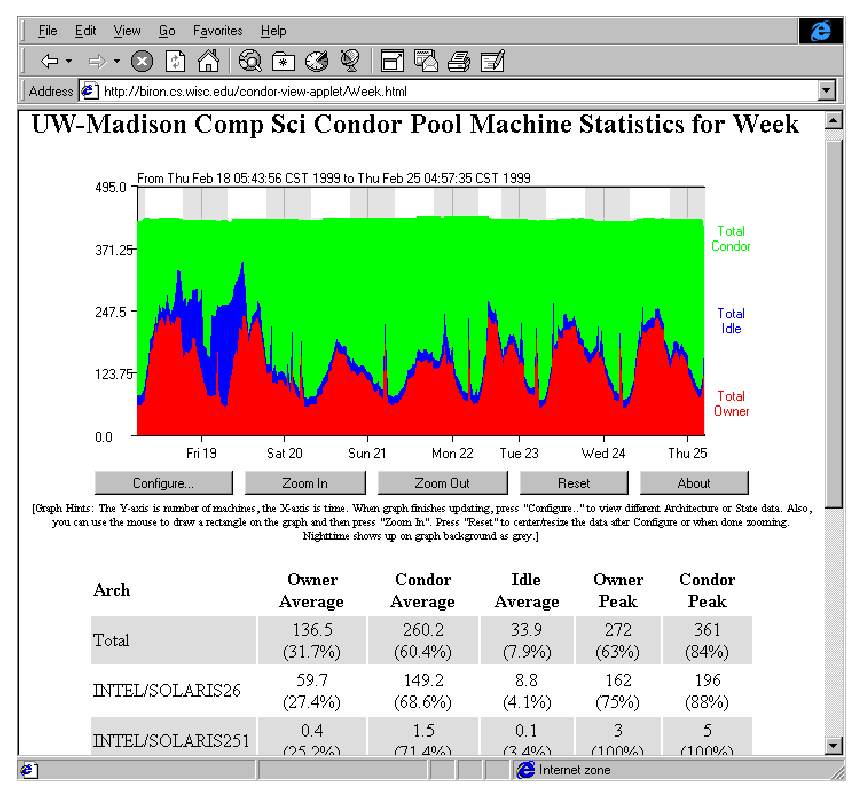
\includegraphics{admin-man/view-screenshot.ps}
\caption{\label{fig:view-screenshot}Screenshot of CondorView Client}
\end{figure}

After unpacking and installing the CondorView Client, a script named
\MakeStats\ can be invoked to create HTML pages displaying Condor usage
for the past hour, day, week, or month.  
By using the Unix \Prog{cron} facility to periodically execute
\MakeStats, Condor pool usage statistics can be kept up to date
automatically.  
This simple model allows the CondorView Client to be installed easily;
no Web server CGI interface is needed.

%%%%%%%%%%%%%%%%%%%%%%%%%%%%%%%%%%%%%%%%%%%%%%%%%%%%%%%%%%%%%%%%%%%%%%
\subsubsection{\label{sec:condorview-client-step-by-step}
Step-by-step installation of the CondorView Client}
%%%%%%%%%%%%%%%%%%%%%%%%%%%%%%%%%%%%%%%%%%%%%%%%%%%%%%%%%%%%%%%%%%%%%%

\begin{enumerate}

\item First, make certain that you have configured your pool's
\Condor{collector} (typically running on the central manager) to log
information to disk in order to provide a persistent, historical
database of pool statistics.  
The CondorView Client makes queries over the network against this
database.  The \Condor{collector} included with version 6.0.x of Condor
does not have this database support; you will need to download and
install the CondorView Server contrib module.  
If you are running Condor
version 6.1 or above, there is no need to install the CondorView Server
contrib module because the \Condor{collector} included in Condor v6.1+
already has the necessary database support.  
To activate the persistent database logging, add the following entries into
the \condor{config} files on your central manager: 
\begin{verbatim}
    POOL_HISTORY_DIR = /full/path/to/directory/to/store/historical/data 
    KEEP_POOL_HISTORY = True 
\end{verbatim}
For full details on these and other \condor{collector} config file
entries, see section~\ref{sec:Collector-Config-File-Entries} on
page~\pageref{sec:Collector-Config-File-Entries}.

\item Create a directory where you would like CondorView to create the
HTML files.  
This directory should be one "published" by a web server, so that HTML
files which exist in this directory can be accessed via a web browser.  
We will refer to this directory as the \emph{VIEWDIR} directory.

\item Unpack/untar the CondorView Client contrib module into the VIEWDIR.
This will create several files and subdirectories in the VIEWDIR.

\item Edit the file \MakeStats.  At the top of this file are six parameters
you need to customize.  The parameters are:

\begin{description}

	\item[\Macro{ORGNAME}] Set to be a very brief name identifying
	your organization, for example ``Univ of Wisconsin''.  Do not
	use any slashes in the name or other special regular-expression
	characters, i.e. avoid characters like: / $\backslash$ \^\ \$.

	\item[\Macro{CONDORADMIN}] Set to the email
	address of the Condor administrator at your site.  
	This email address will appear at the bottom of the web pages.

	\item[\Macro{VIEWDIR}] Set to the full pathname
	(\Bold{not} a relative path) to the VIEWDIR directory you selected
	in installation step \#2 above.  
	It is the same directory where the \MakeStats\ file lives.

	\item[\Macro{STATSDIR}]  Set to the full
	pathname of the \Bold{directory} which contains the \Condor{stats}
	binary.  
	The \Condor{stats} program is included in the \Release{bin}
	directory with Condor version 6.1 and above; for Condor version
	6.0x, the \Condor{stats} program can be found in the CondorView
	Server contrib module.  
	The value for \Macro{STATSDIR} is added to the \Macro{PATH}
	parameter by default; see below.  

	\item[\Macro{PATH}] Set to a list of subdirectories,
	separated by colons, where the \MakeStats\ script can find
	\Prog{awk}, \Prog{bc}, \Prog{sed}, \Prog{date}, and \Condor{stats}
	programs.  
	If you have \Prog{perl} installed on this system, set the path to
	include the directory where \Prog{perl} is installed as well.  Using
	the below default works on most systems:
\begin{verbatim} 
        PATH=/bin:/usr/bin:$STATSDIR:/usr/local/bin
\end{verbatim}

\end{description}

	\item Now type: 
\begin{verbatim}
        ./make_stats setup  
\end{verbatim}
	This will create all of the initial HTML files.  Open up the file
	\File{index.html} and verify things look good.

	\item Add the \MakeStats\ program to cron.  Running ``\MakeStats\ 
	setup'' in step 5 should have created a \File{cronentries} file.
	This \File{cronentries} file is ready to be processed by your Unix
	system's \Prog{crontab} command.  Enter ``man crontab'' on your
	system if you are not familiar with the \Prog{crontab} command
	and/or the \Prog{cron} daemon.  Take a look at the
	\File{cronentries} file; by default, it will run ``\MakeStats\ hour''
	every 15 minutes, ``\MakeStats\ day'' once an hour, ``\MakeStats\ 
	week'' twice per day, and ``\MakeStats\ month'' once per day.  These
	are reasonable defaults.  You can add these commands to cron on any
	system that can access to the \MacroU{VIEWDIR} and
	\MacroU{STATSDIR}, even on a system that does not have Condor
	installed.  The commands do not have to run as user root either; in
	fact, they should probably not run as root.  These commands can run
	as any user that has read/write access to the VIEWDIR.  To add these
	commands to cron, enter : 
\begin{verbatim} 
        crontab cronentries
\end{verbatim}

	\item That's it!  Point your web browser at the VIEWDIR directory,
	and you should be all set.

\end{enumerate}


%%%%%%%%%%%%%%%%%%%%%%%%%%%%%%%%%%%%%%%%%%%%%%%%%%%%%%%%%%%%%%%%%%%%%%
\section{\label{sec:Ckpt-Server} The Checkpoint Server}
%%%%%%%%%%%%%%%%%%%%%%%%%%%%%%%%%%%%%%%%%%%%%%%%%%%%%%%%%%%%%%%%%%%%%%

\index{installation!checkpoint server}
\index{checkpoint server!installation|(}
\index{HTCondor daemon!condor\_ckpt\_server@\Condor{ckpt\_server}}
\index{daemon!condor\_ckpt\_server@\Condor{ckpt\_server}}
\index{condor\_ckpt\_server daemon}
A Checkpoint Server maintains a repository for checkpoint files.
Within HTCondor, checkpoints may be produced only for standard universe jobs.
Using checkpoint servers reduces the disk requirements of submitting
machines in the pool, since the submitting machines no longer need to
store checkpoint files locally.
Checkpoint server machines should have a large amount of disk space
available, and they should have a fast connection to machines
in the HTCondor pool.

If the spool directories are on a network file system, then
checkpoint files will make two trips over the network: one between the
submitting machine and the execution machine, and a second between the
submitting machine and the network file server.
A checkpoint server configured to use the server's local disk
means that the checkpoint file will travel only once over the
network, between the execution machine and the checkpoint server.
The pool may also obtain checkpointing network performance benefits by
using multiple checkpoint servers, as discussed below.

Note that it is a good idea to pick very stable machines for the checkpoint
servers.
If individual checkpoint servers crash, the HTCondor system will continue to
operate, although poorly.  
While the HTCondor system will recover from a checkpoint server crash
as best it can, there are two problems that can and will occur:
\begin{enumerate}

\item A checkpoint cannot be sent to a checkpoint server that
is not functioning.
Jobs will keep trying to contact the checkpoint server, backing
off exponentially in the time they wait between attempts.
Normally, jobs only have a limited time to checkpoint before they are
kicked off the machine.
So, if the checkpoint server is down for a long period of time,
chances are that a lot of work will be lost by jobs being killed 
without writing a checkpoint. 

\item If a checkpoint is not available from the checkpoint server,
a job cannot be retrieved, and it will either have to be restarted from
the beginning, or the job will wait for the server to come back on line.
This behavior is controlled with the
\Macro{MAX\_DISCARDED\_RUN\_TIME} configuration variable.
This variable represents the maximum amount of CPU time the job is
willing to discard, by starting a job over from its beginning if the
checkpoint server is not responding to requests.

\end{enumerate}

%%%%%%%%%%%%%%%%%%%%%%%%%%%%%%%%%%%%%%%%%%%%%%%%%%%%%%%%%%%%%%%%%%%%%%
\subsection{\label{Prepare-Ckpt-Server} Preparing to Install
a Checkpoint Server} 
%%%%%%%%%%%%%%%%%%%%%%%%%%%%%%%%%%%%%%%%%%%%%%%%%%%%%%%%%%%%%%%%%%%%%%

The location of checkpoint files changes upon the installation
of a checkpoint server.
A configuration change will cause 
currently queued jobs with checkpoints
to not be able to find their checkpoints.
This results in the jobs with checkpoints
remaining indefinitely queued,
due to the lack of finding their checkpoints.
It is therefore best to 
either remove jobs from the queues or let them complete
before installing a checkpoint server.
It is advisable to shut the pool down before doing any
maintenance on the checkpoint server.  
See section~\ref{sec:Pool-Management} on
page~\pageref{sec:Pool-Management} for details on shutting
down the pool. 

A graduated installation of the checkpoint server may be
accomplished by 
configuring submit machines as their queues empty.

%%%%%%%%%%%%%%%%%%%%%%%%%%%%%%%%%%%%%%%%%%%%%%%%%%%%%%%%%%%%%%%%%%%%%%
\subsection{\label{Install-Ckpt-Server-Module}
Installing the Checkpoint Server Module} 
%%%%%%%%%%%%%%%%%%%%%%%%%%%%%%%%%%%%%%%%%%%%%%%%%%%%%%%%%%%%%%%%%%%%%%

The files relevant to a checkpoint server are
\begin{verbatim}
        sbin/condor_ckpt_server
        etc/examples/condor_config.local.ckpt.server
\end{verbatim}

\File{\condor{ckpt\_server}} is the checkpoint server binary.
\File{\condor{condor\_config.local.ckpt.server}} is an example
configuration for a checkpoint server. The settings embodied in this
file must be customized with site-specific information.

There are three steps necessary towards running a checkpoint server:
\begin{enumerate}
\item Configure the checkpoint server.
\item Start the checkpoint server.
\item Configure the pool to use the checkpoint server.
\end{enumerate}


\begin{description}

\item[Configure the Checkpoint Server]

\index{checkpoint server!configuration of}
Place settings in the local configuration file of
the checkpoint server.
The file \File{etc/examples/condor\_config.local.ckpt.server} contains
a template for the needed configuration. Insert these into the local
configuration file of the checkpoint server machine. 

The value of \Macro{CKPT\_SERVER\_DIR}  
must be customized.
This variable defines the location of checkpoint files.
It is better if this location is within a very fast local file system,
and preferably a RAID. 
The speed of this file system will have a direct impact on the speed
at which checkpoint files can be retrieved from the remote machines. 

The other optional variables are:
\begin{description}

\item[\Macro{DAEMON\_LIST}] Described in
section~\ref{sec:Master-Config-File-Entries}.  
To have the checkpoint server managed by the \Condor{master},
the \MacroNI{DAEMON\_LIST} variable's value must list both \Expr{MASTER}
and \Expr{CKPT\_SERVER}.
Also add \Expr{STARTD} to allow jobs to run on the checkpoint server machine.
Similarly, add \Expr{SCHEDD} to permit the submission of jobs from the
checkpoint server machine. 

\end{description}

The remainder of these variables are the checkpoint server-specific versions
of the HTCondor logging entries, as described in
section~\ref{sec:Daemon-Logging-Config-File-Entries} on
page~\pageref{sec:Daemon-Logging-Config-File-Entries}.
\begin{description}

\item[\Macro{CKPT\_SERVER\_LOG}] The location of the checkpoint server log.

\item[\Macro{MAX\_CKPT\_SERVER\_LOG}] Sets the maximum
size of the checkpoint server log, before it is saved and the
log file restarted.

\item[\Macro{CKPT\_SERVER\_DEBUG}] Regulates the amount of information
printed in the log file.
Currently, the only debug level supported is \Dflag{ALWAYS}.

\end{description}

\item[Start the Checkpoint Server]

To start the newly configured checkpoint server,
restart HTCondor on that host to enable
the \Condor{master} to notice the new configuration.
Do this by sending a \Condor{restart} command from any machine
with administrator access to the pool.
See section~\ref{sec:Host-Security} on
page~\pageref{sec:Host-Security} for full details about IP/host-based
security in HTCondor. 

Note that when the \Condor{ckpt\_server} starts up, it will immediately
inspect any checkpoint files in the location described by the
\MacroNI{CKPT\_SERVER\_DIR} variable, and determine if any of them are stale.
Stale checkpoint files will be removed.

\item[Configure the Pool to Use the Checkpoint Server]

After the checkpoint server is running,
modify a few configuration variables to let the other machines in the pool
know about the new server:

\begin{description}
   \item[\Macro{USE\_CKPT\_SERVER}] A boolean value that should be set to
   \Expr{True} to enable the use of the checkpoint server.

   \item[\Macro{CKPT\_SERVER\_HOST}] Provides the full host name 
   of the machine that is now running the checkpoint server.  
\end{description}

It is most convenient to set these variables in the pool's
global configuration file,
so that they affect all submission machines.
However, it is permitted to configure each submission machine separately
(using local configuration files), for example if it is desired that not all
submission machines begin using the checkpoint server at one time.
If the variable \MacroNI{USE\_CKPT\_SERVER} is set to \Expr{False},
the submission machine will not use a checkpoint server.

Once these variables are in place,
send the command \Condor{reconfig} to all machines in the pool,
so the changes take effect.
This is described in section~\ref{sec:Reconfigure-Pool} on
page~\pageref{sec:Reconfigure-Pool}.

\end{description}

%%%%%%%%%%%%%%%%%%%%%%%%%%%%%%%%%%%%%%%%%%%%%%%%%%%%%%%%%%%%%%%%%%%%%%
\subsection{\label{Configure-Multiple-Ckpt-Server} 
Configuring the Pool to Use Multiple Checkpoint Servers}
%%%%%%%%%%%%%%%%%%%%%%%%%%%%%%%%%%%%%%%%%%%%%%%%%%%%%%%%%%%%%%%%%%%%%%

\index{checkpoint server!multiple servers}

An HTCondor pool may use multiple checkpoint servers.
The deployment of
checkpoint servers across the
network improves the performance of checkpoint production.
In this case, HTCondor machines are configured to send checkpoints to the
\emph{nearest} checkpoint server.
There are two main performance benefits to deploying multiple checkpoint
servers:
\begin{itemize}
\item Checkpoint-related network traffic is localized by
intelligent placement of checkpoint servers.
\item Better performance implies that jobs spend less time
dealing with checkpoints, and more time doing useful work,
leading to jobs having a higher success rate before returning a
machine to its owner, and workstation
owners see HTCondor jobs leave their machines quicker.
\end{itemize}

With multiple checkpoint servers running in the pool, the
following configuration changes are required to make them active.

Set \Macro{USE\_CKPT\_SERVER} to \Expr{True} (the default) on all
submitting machines where HTCondor jobs should use a checkpoint server.
Additionally, variable \Macro{STARTER\_CHOOSES\_CKPT\_SERVER} should be set to
\Expr{True} (the default) on these submitting machines.
When \Expr{True}, this variable specifies that the checkpoint server
specified by the machine running the job should be used instead of the
checkpoint server specified by the submitting machine.
See section~\ref{sec:Checkpoint-Server-Config-File-Entries} on
page~\pageref{sec:Checkpoint-Server-Config-File-Entries} for more
details.
This allows the job to use the checkpoint server closest to the
machine on which it is running, instead of the server closest to the
submitting machine.
For convenience, set these parameters in the
global configuration file.

Second, set \Macro{CKPT\_SERVER\_HOST} on each machine.
This identifies the full host name of the checkpoint server machine,
and should be the host name of the nearest server to the machine.
In the case of multiple checkpoint servers, set this
in the local configuration file.

Third, send a
\Condor{reconfig} command to all machines in the pool, 
so that the changes take effect.
This is described in section~\ref{sec:Reconfigure-Pool} on
page~\pageref{sec:Reconfigure-Pool}.

After completing these three steps, the jobs in the pool will
send their checkpoints to the nearest checkpoint server.
On restart, a job will remember where its checkpoint was
stored and retrieve it from the appropriate server.
After a job successfully writes a checkpoint to a new server, it will
remove any previous checkpoints left on other servers.

Note that if the configured checkpoint server is unavailable,
the job will keep trying to contact that server.
It will not use alternate checkpoint servers.
This may change in future versions of HTCondor.

%%%%%%%%%%%%%%%%%%%%%%%%%%%%%%%%%%%%%%%%%%%%%%%%%%%%%%%%%%%%%%%%%%%%%%
\subsection{\label{Checkpoint-Server-Domains} 
Checkpoint Server Domains}
%%%%%%%%%%%%%%%%%%%%%%%%%%%%%%%%%%%%%%%%%%%%%%%%%%%%%%%%%%%%%%%%%%%%%%

The configuration described in the previous section ensures that jobs
will always write checkpoints to their nearest checkpoint server.  In
some circumstances, it is also useful to configure HTCondor to localize
checkpoint read transfers, which occur when the job restarts from its
last checkpoint on a new machine.  To localize these transfers, 
it is desired
to schedule the job on a machine which is near the checkpoint
server on which the job's checkpoint is stored.

In terminology, all of the machines configured to use checkpoint
server \Term{A} are in \Term{checkpoint server domain A}.
To localize checkpoint transfers, 
jobs which run on machines in a given
checkpoint server domain should continue running on machines in that domain,
thereby transferring checkpoint files in a single local area of the network.
There are two possible configurations which specify what a
job should do when there are no available machines in its checkpoint
server domain:
\begin{itemize}
\item The job can remain idle until a workstation in its checkpoint
server domain becomes available.
\item The job can try to immediately begin executing on a machine
in another checkpoint server domain.  In this case, the job transfers
to a new checkpoint server domain.
\end{itemize}
These two configurations are described below.

The first step in implementing checkpoint server domains is to include
the name of the nearest checkpoint server in the machine
ClassAd, so this information can be used in job scheduling decisions.
To do this, add the following configuration to each machine:
\begin{verbatim}
  CkptServer = "$(CKPT_SERVER_HOST)"
  STARTD_ATTRS = $(STARTD_ATTRS), CkptServer
\end{verbatim}
For convenience, set these variables in the global configuration file.
Note that this example assumes that
\MacroNI{STARTD\_ATTRS} is previously defined in the configuration.
If not, then use the following configuration instead:
\begin{verbatim}
  CkptServer = "$(CKPT_SERVER_HOST)"
  STARTD_ATTRS = CkptServer
\end{verbatim}
With this configuration, all machine ClassAds will include a \AdAttr{CkptServer}
attribute, which is the name of the checkpoint server closest to this
machine.  So, the \AdAttr{CkptServer} attribute defines the checkpoint
server domain of each machine.

To restrict jobs to one checkpoint server domain,
modify the jobs' \AdAttr{Requirements} expression as follows:
\footnotesize
\begin{verbatim}
  Requirements = ((LastCkptServer == TARGET.CkptServer) || (LastCkptServer =?= UNDEFINED))
\end{verbatim}
\normalsize
This \AdAttr{Requirements} expression uses the \AdAttr{LastCkptServer}
attribute in the job's ClassAd, which specifies where the job last
wrote a checkpoint, and the \AdAttr{CkptServer} attribute in the
machine ClassAd, which specifies the checkpoint server domain.  If the
job has not yet written a checkpoint, the \AdAttr{LastCkptServer}
attribute will be \Expr{Undefined}, and the job will be able to execute in
any checkpoint server domain.  However, once the job performs a
checkpoint,
\AdAttr{LastCkptServer} will be defined and the job will be restricted to the
checkpoint server domain where it started running.

To instead allow jobs to transfer to other checkpoint
server domains when there are no available machines in the current
checkpoint server domain, modify the jobs' \AdAttr{Rank} expression
as follows:
\footnotesize
\begin{verbatim}
  Rank = ((LastCkptServer == TARGET.CkptServer) || (LastCkptServer =?= UNDEFINED))
\end{verbatim}
\normalsize
This \AdAttr{Rank} expression will evaluate to 1 for machines in the
job's checkpoint server domain and 0 for other machines.  So, the job
will prefer to run on machines in its checkpoint server domain, but if
no such machines are available, the job will run in a new checkpoint
server domain.

The checkpoint server domain \AdAttr{Requirements} or \AdAttr{Rank} expressions 
can be automatically appended 
to all standard universe jobs submitted in the pool using
the configuration variables
\MacroNI{APPEND\_REQ\_STANDARD} or \MacroNI{APPEND\_RANK\_STANDARD}.
See section~\ref{sec:Submit-Config-File-Entries} on
page~\pageref{sec:Submit-Config-File-Entries} for more details.
\index{checkpoint server!installation|)}

%%%%%%%%%%%%%%%%%%%%%%%%%%%%%%%%%%%%%%%%%%%%%%%%%%%%%%%%%%%%%%%%%%%%%%
\subsection{Installing PVM Support in Condor}
\label{sec:Install-PVM-Condor}
%%%%%%%%%%%%%%%%%%%%%%%%%%%%%%%%%%%%%%%%%%%%%%%%%%%%%%%%%%%%%%%%%%%%%%

\Todo


%%%%%%%%%%%%%%%%%%%%%%%%%%%%%%%%%%%%%%%%%%%%%%%%%%%%%%%%%%%%%%%%%%%%%%
\subsection{\label{sec:EventD}
Condor Event Daemon}
%%%%%%%%%%%%%%%%%%%%%%%%%%%%%%%%%%%%%%%%%%%%%%%%%%%%%%%%%%%%%%%%%%%%%%

\index{daemon!eventd}
\index{event daemon}
\index{contrib module!event daemon}

The event daemon is an administrative tool for scheduling events in a
Condor pool.
Every \Macro{EVENTD\_INTERVAL}, for each defined event, the event
daemon (eventd) computes an estimate of the time required to complete or
prepare for the event.  If the time required is less than the time
between the next interval and the start of the event, the event daemon
activates the event.

Currently, this daemon supports \Macro{SHUTDOWN} events, which place machines
in the owner state during scheduled times.
The eventd causes machines to vacate jobs one at a time
in anticipation of \Macro{SHUTDOWN} events.
Scheduling this improves performance, because the machines
do not all attempt to checkpoint their jobs at the same time.
To determine the estimate of the time required to complete a \Macro{SHUTDOWN}
event, the \Attr{ImageSize} values for all running standard universe jobs are
totalled and then divided by the maximum bandwidth specified for this
event.

When a \Macro{SHUTDOWN} event is activated, the eventd contacts all startd
daemons
that match constraints given in the configuration file,
and instructs them to shut down.
In response to this instruction,
the startd on any machine not running a job will immediately transition to
the owner state.
Any machine currently running a job will continue to run the
job, but will not start any new job.
The eventd then sends a vacate command to the each startd
that is currently running a job.
Once the job is vacated, the startd transitions to the
owner state.

\Condor{eventd} must run on a machine with administrator
access to your pool.
See section~\ref{sec:Host-Security} on
page~\pageref{sec:Host-Security} for full details about IP/host-based
security in Condor.

%%%%%%%%%%%%%%%%%%%%%%%%%%%%%%%%%%%%%%%%%%%%%%%%%%%%%%%%%%%%%%%%%%%%%%
\subsubsection{\label{sec:EventD-Installation}
Installing the Event Daemon} 
%%%%%%%%%%%%%%%%%%%%%%%%%%%%%%%%%%%%%%%%%%%%%%%%%%%%%%%%%%%%%%%%%%%%%%

\Condor{eventd} requires version 6.1.3 or later of
\Condor{startd}.
So, you should first install either the latest version of the SMP
\Condor{startd} contrib module or the latest release of Condor version
6.1.

First, download the \Condor{eventd} contrib module.
Uncompress and untar the file, to have a directory that
contains a \File{eventd.tar}.
The \File{eventd.tar} acts much like the \File{release.tar} file from
a main release.
This archive contains the files:
\begin{verbatim}
	sbin/condor_eventd
	etc/examples/condor_config.local.eventd
\end{verbatim}
These are all new files, not found in the main release, so you can
safely untar the archive directly into your existing release
directory.
The file \File{\condor{eventd}} is the eventd binary.
The example configuration file is described below.

%%%%%%%%%%%%%%%%%%%%%%%%%%%%%%%%%%%%%%%%%%%%%%%%%%%%%%%%%%%%%%%%%%%%%%
\subsubsection{\label{sec:EventD-Configuration}
Configuring the Event Daemon} 
%%%%%%%%%%%%%%%%%%%%%%%%%%%%%%%%%%%%%%%%%%%%%%%%%%%%%%%%%%%%%%%%%%%%%%

The file \File{etc/examples/condor\_config.local.eventd} contains an
example configuration.
To define events, first set the \Macro{EVENT\_LIST} macro.
This macro contains a list of macro names which define the individual
events.
The definition of individual events depends on the type of the event.
Currently, there is only one event type: \Macro{SHUTDOWN}.
The format for \Macro{SHUTDOWN} events is
\begin{verbatim}
	SHUTDOWN DAY TIME DURATION BANDWIDTH CONSTRAINT RANK
\end{verbatim}
\verb@TIME@ and \verb@DURATION@ are specified in an hours:minutes format.

For example:
\index{event daemon!example configuration}
\begin{verbatim}
EVENT_LIST	= TestEvent, TestEvent2
TestEvent	= SHUTDOWN W 16:00 1:00 2.5 TestEventConstraint TestEventRank
TestEvent2	= SHUTDOWN F 14:00 0:30 6.0 TestEventConstraint2 TestEventRank
TestEventConstraint		= (Arch == "INTEL")
TestEventConstraint2		= (True)
TestEventRank			= (0 - ImageSize)
\end{verbatim}

In this example, the \verb@TestEvent@ is a \Macro{SHUTDOWN} type event, which
specifies that all machines whose startd ads match the constraint
\verb@Arch == "INTEL"@ should be shutdown for one hour starting at
16:00 every Wednesday, and no more than 2.5 Mbytes/s of bandwidth
should be used to vacate jobs in anticipation of the shutdown
event.  According to the \verb@TestEventRank@, jobs will be vacated in
reverse order of their \Attr{ImageSize} (larger jobs first, smaller jobs
last).  \verb@TestEvent2@ is a \Macro{SHUTDOWN} type event, which specifies
that all machines should be shutdown for 30 minutes starting at
14:00 every Friday, and no more than 6.0 Mbytes/s of bandwidth should
be used to vacate jobs in anticipation of the shutdown event.

Note that the \Macro{DAEMON\_LIST} macro (described in
section~\ref{sec:Master-Config-File-Entries}) is defined in the
section of settings you may want to customize.
If you want the event daemon managed by the \Condor{master}, the
\Macro{DAEMON\_LIST} entry must contain both 
\Attr{MASTER} and \Attr{EVENTD}.
Verify that this macro is set to run the correct daemons on
this machine.  By default, the list also includes
\Attr{SCHEDD} and \Attr{STARTD}.

See section~\ref{sec:Eventd-Config-File-Entries} on
page~\pageref{sec:Eventd-Config-File-Entries} for a description of
optional event daemon parameters.

%%%%%%%%%%%%%%%%%%%%%%%%%%%%%%%%%%%%%%%%%%%%%%%%%%%%%%%%%%%%%%%%%%%%%%
\subsubsection{\label{sec:Start-EventD} 
Starting the Event Daemon} 
%%%%%%%%%%%%%%%%%%%%%%%%%%%%%%%%%%%%%%%%%%%%%%%%%%%%%%%%%%%%%%%%%%%%%%

To start an event daemon once it is configured to run on a given
machine, restart Condor on that given machine to enable
the \Condor{master} to notice the new configuration.
Send a \Condor{restart} command from any machine
with administrator access to your pool.
See section~\ref{sec:Host-Security} on
page~\pageref{sec:Host-Security} for full details about IP/host-based
security in Condor.






